\par
\vspace{0.3cm}
\noindent
\textit{\textbf{Simultaneous Drilling of Horizontal Wells with Heterogeneous Geological Qualities}} ---
Figure \ref{Figure:Simultaneous-Drilling-of-Horizontal-Wells-with-Heterogeneous-Geological-Quality}, summarizing the estimated geological qualities of horizontal wells in scatter plots, clearly demonstrates that horizontal wells with a range of geological qualities were drilled simultaneously in the Bakken region of North Dakota. And as shown in Figure \ref{Figure:High-Sensitivity-of-Firm-Level-Low-Quality-Well-Drilling}, simultaneous drilling is observed even at the firm level. 

\afterpage{
    \begin{figure}[t!]
        \centering
        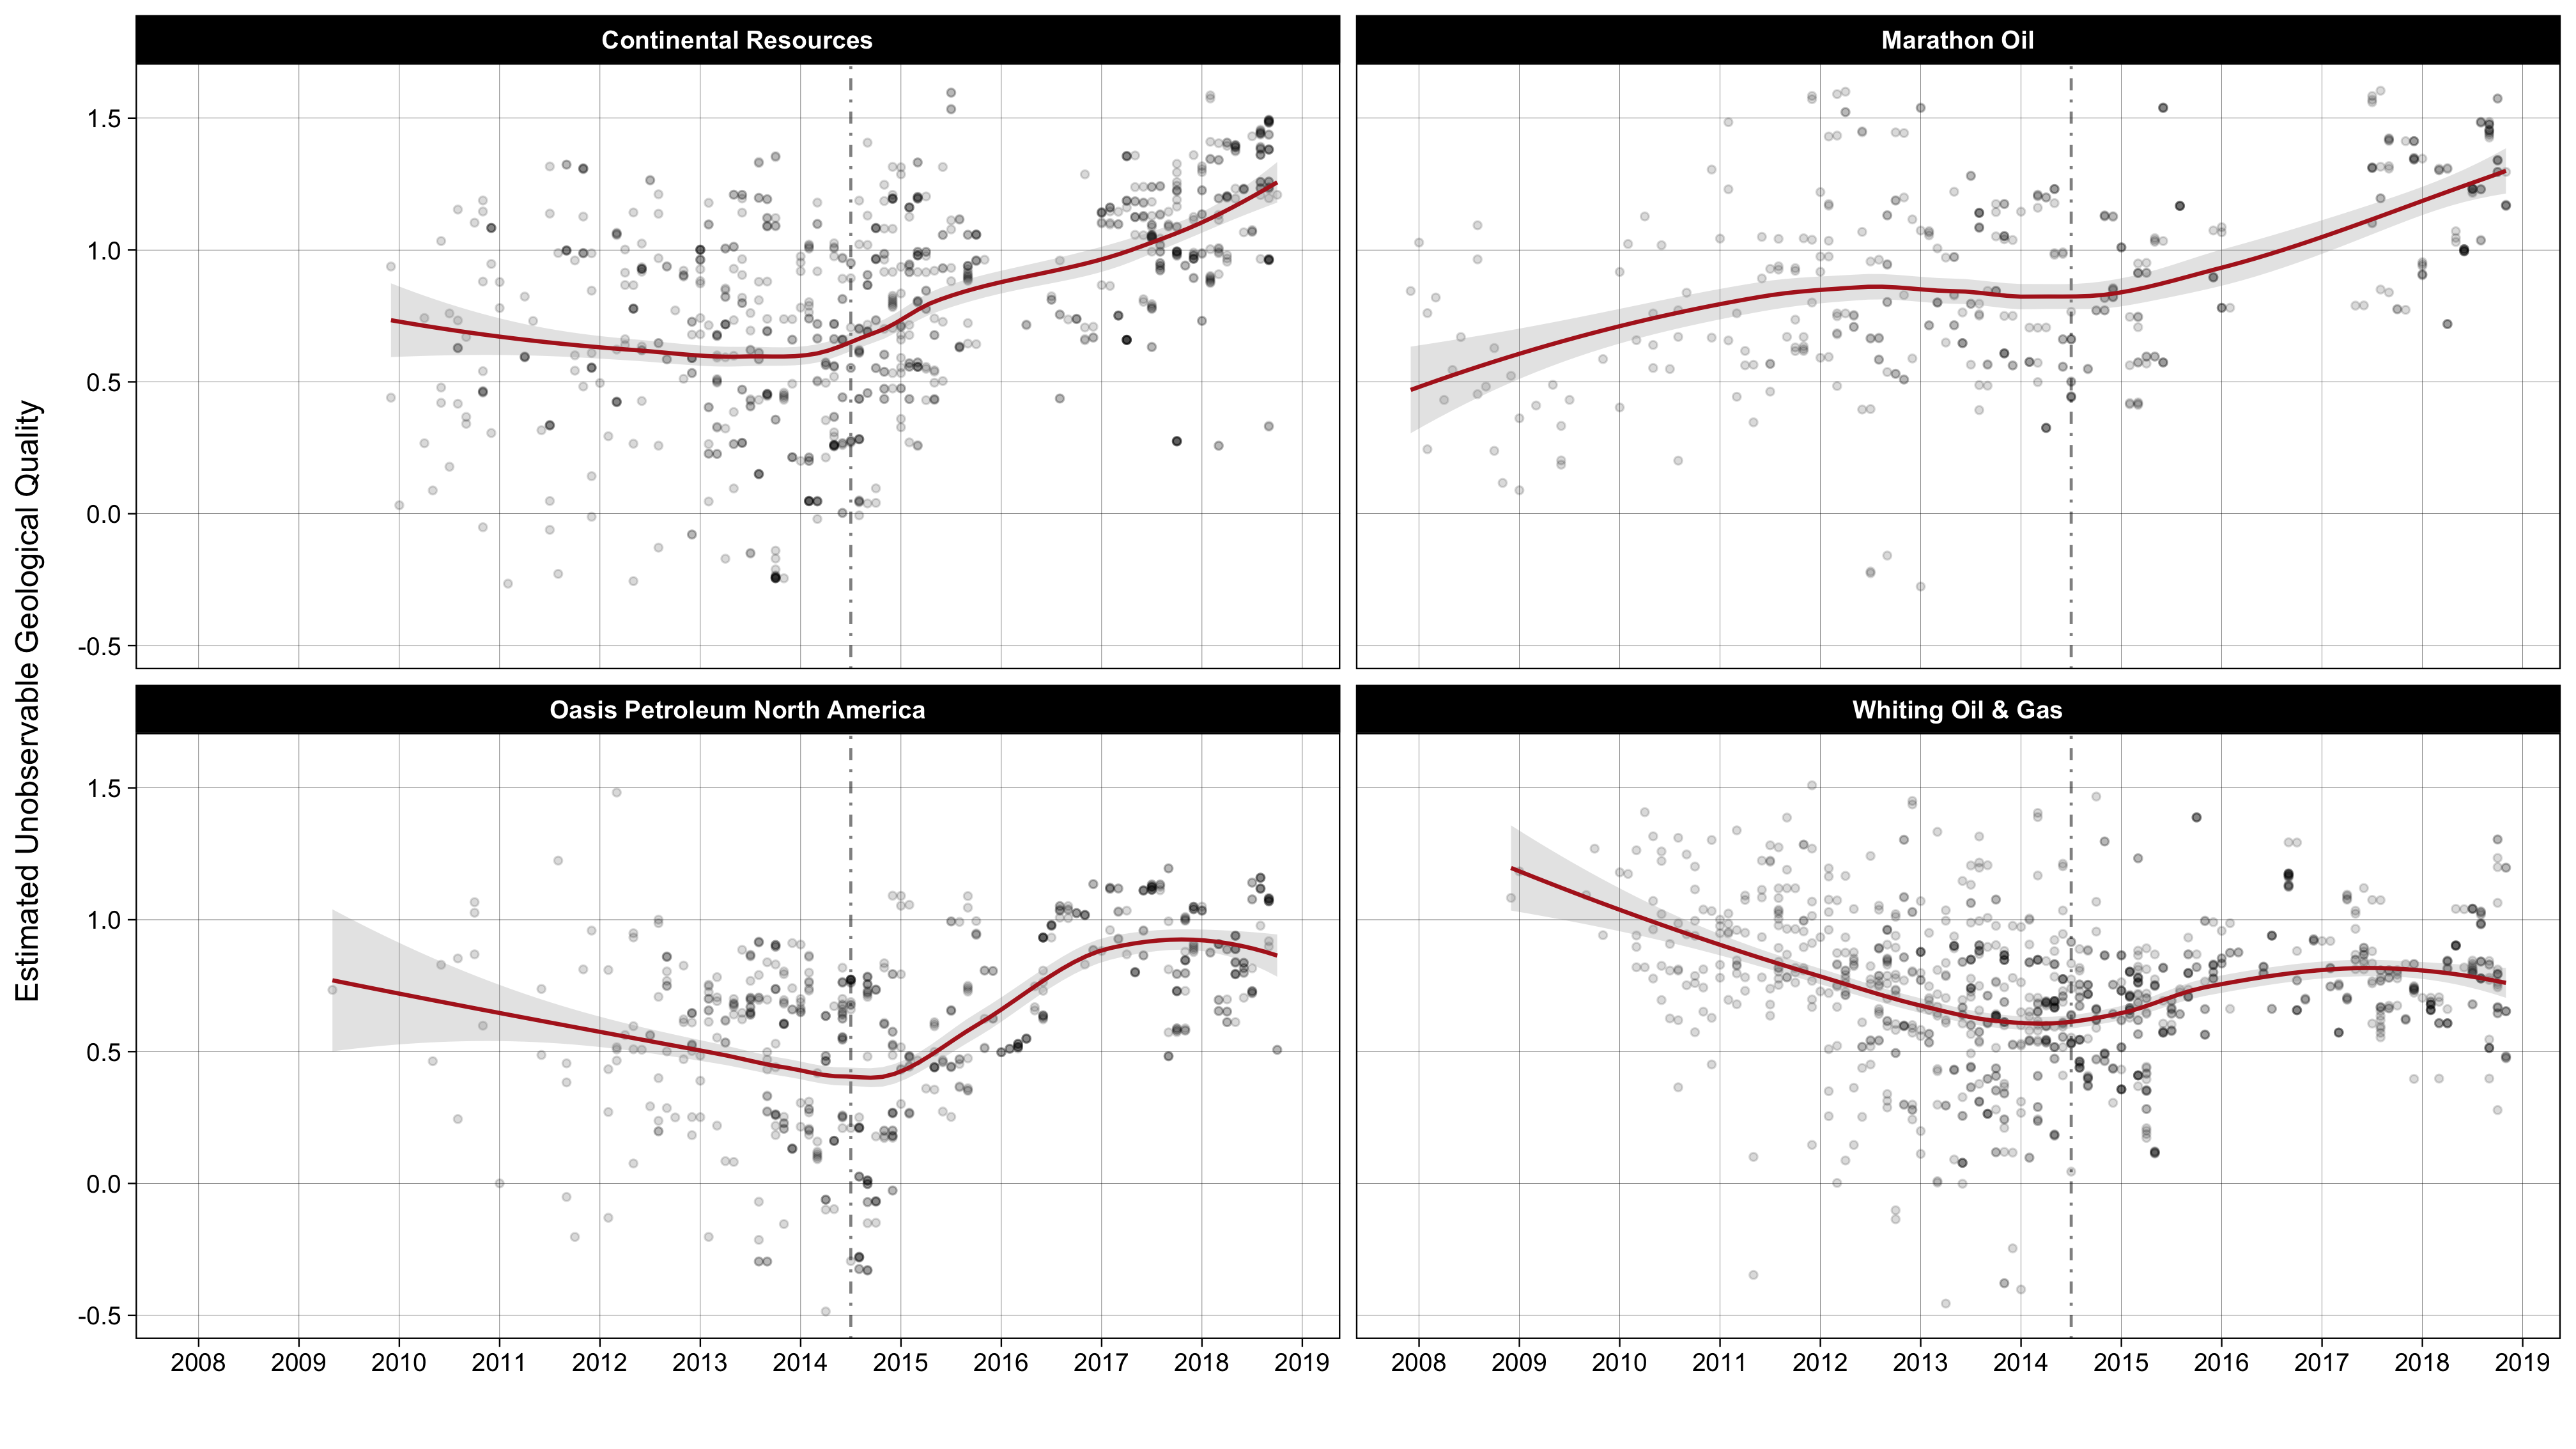
\includegraphics[scale = 0.11]{04_Chapter-3/00A_Figures/Figure_Cross-Sectional-Approach_Estimates-from-Robinson-Estimator_Time-Trend-of-Unobservable-Geological-Quality_Firms.png}
        \caption{High Sensitivity of Firm-Level Low-Quality Well Drilling to the Negative Price Shocks in 2014-15}
        \caption*{
            {\small
            \textit{Note}: 
            This figure shows how the four firms' drilling activity changed over time. Each dot in the figure indicates an individual well's estimated geological feature. The red line, with the 95\% confidence interval, in each panel demonstrates the average quality of horizontal wells drilled in a month. As illustrated, the firms significantly reduced drilling low-quality well locations since mid-2014, corresponding to the beginning of the oil price plunge.
        }}
        \label{Figure:High-Sensitivity-of-Firm-Level-Low-Quality-Well-Drilling}
    \end{figure}
}
Simultaneous drilling of both low- and high-quality resources contradicts the well-known least-cost-first extraction rule in nonrenewable resource extraction.\footnote{The cost that matters here is the marginal cost. And the marginal cost consists of two distinct costs: the marginal cost of drilling a new well and the marginal cost of extracting oil from existing wells.} According to the rule derived from the canonical Hotelling model, deposits of an exhaustible resource should be exploited in strict order, beginning with the lowest cost deposit.\footnote{See \textit{Selection 7 Depletion and Economic Theory} in \cite{Resource-Economics_Brooks_2015}.} Because a larger estimate of the unobservable geological quality implies higher ultimate oil production, if the rule holds, wells with larger estimates, thus having lower per-barrel marginal cost, should be first extracted. Those figures, however, do not show the theoretical prediction at all. 
